%%This is a very basic article template.
%%There is just one section and two subsections.
\documentclass[12pt, a4paper]{report}
\linespread{1.5}
%%\pagestyle{headings}
\usepackage{fancyhdr}   
\usepackage{graphicx} 
\pagestyle{fancy}          
%zmianaliterw~ywejpaginienamae
\renewcommand{\chaptermark}[1]{\markboth{#1}{}}
\renewcommand{\sectionmark}[1]{\markright{\thesection\#1}}
\fancyhf{}%usubie�ceustawieniapagin 
\fancyhead[LE,RO]{\small\bfseries\thepage}
\fancyhead[LO]{\small\bfseries\rightmark} 
\fancyhead[RE]{\small\bfseries\leftmark}
\renewcommand{\headrulewidth}{0.5pt} 
\addtolength{\headheight}{0.5pt}%pionowyodstpnakresk
\fancypagestyle{plain}{%  
\fancyhead{}%usup.g�rnenastronachpozbawionych 
%numeracji(plain) 
\renewcommand{\headrulewidth}{0pt}%poziomakreska
}
\usepackage{graphicx}  
\usepackage{polski}
\usepackage[cp1250]{inputenc}
%%\includeonly{chapter1,chapter2, bibliography}
\begin{document}
\title{Integracja technologii mobilnych i system�w klasy Enterprise}
\author{Wojciech Klicki 	\and Konrad Starzyk}
\date{}
\maketitle
\tableofcontents
\clearpage 

\chapter{Integracja w �rodowiskach Enterprise }
 
\section{Istniej�ce podej�cia do integracji}
W zale�no�ci od system�w kt�re integrujemy, czy to jest jedna rozproszona
aplikacja czy wiele niezale�nych komponent�w musimy zdecydowa� si� na jedno z
rowi�za� integracyjnych. Rozwa�aj�c mo�liwe sposoby integracji technologii
mobilnych z rozbudowan� aplikacj� klasy enteprise musimy zwr�ci� uwag� na
udost�pniane z obu stron mechanizmy.
\subsection{Transfer plik�w}
W tym przypadku dane s� zapisywane i odczytywane z plik�w. Niezb�dna jest
wsp�lna przestrze� dyskowa lub spos�b przesy�ania (np. FTP). Z tego powodu
musimy odrzuci� takie rozwi�zanie jako niedaj�ce si� zaimplementowa� w
�rodowisku mobilnym.
\subsection{Wsp�lna baza danych}
Dane s� sk�adowane we wsp�lnej bazie danych. Ze wzgl�du na zawodno�� transferu
oraz d�ugi czas przesy�ania danych pomi�dzy urz�dzeniem mobilnym a serwerem, a
tym samym konieczno�� d�ugiego oczekiwania, rezygnujemy z takiego rozwi�zania.
\subsection{RPC}
Zdalne wywo�ywanie procedur (ang. Remote Procedure Call) jest mechanizmem kt�ry
pozwala wykonywa� procedury udost�pniane przez zdalny system. Za�o�eniem
wywo�a� RPC jest synchroniczno��, kt�ra wprawdzie nie oznacza, �e musimy czeka�
na rezultat dzia�ania (mo�emy za�o�y�, �e wy��cznie zlecamy wykonanie
procedury, pobieraj�c wynik potem),ale �e zak�adamy niezawodno�� komunikacji
mi�dzy urz�dzeniami.
\subsection{Wiadomo�ci}
Preferowanym przez nas rozwi�zaniem w takim przypadku jest wykorzystanie
wiadomo�ci. Komunikacja za pomoc� wiadomo�ci jest asynchroniczna, dodatkowo
dobry system przesy�ania wiadomo�ci gwarantuje jej dostarczenie do adresata,
lub informacj� o jej niedostarczeniu. System przesy�ania wiadomo�ci znakomicie
wype�nia luk� komunikacyjn� pomi�dzy systemami klasy Enterprise i urz�dzeniami
mobilnymi. Musimy pami�ta�, �e warunki w jakich mo�emy komunikowa� si� z
urz�dzeniem przeno�nym s� dalekie od doskona�ych, a mimo to u�ytkownik oczekuje
pe�nej niezawodno�ci systemu. To sprawia, �e nale�y go tak zaprojektowa�, aby
przerwy w komunikacji by�y jak najmniej odczuwalne. Systemy komunikacyjne takie
jak RPC,RMI czy CORBA projektowane by�y dla warunk�w w kt�rych problemy
komunikacyjne s� sytuacj� nadzwyczajn�. Tymczasem w przypadku ��czno�ci
bezprzewodowej utrata po��czenia nie jest niczym czego nie mogliby�my si�
spodziewa�. W tym momencie idea przesy�ania wiadomo�ci wydaje si� skutecznym (o
ile nie jedynym) rozwi�zaniem tych problem�w.

\section{Systemy oparte na przesy�aniu wiadomo�ci}
Systemy przesy�ania wiadomo�ci pozwalaj� na integracj� system�w z
uwzgl�dnieniem specyfiki ka�dego z nich. Jednak jak ka�de rozwi�zanie maj�
swoje mocne i s�abe strony.

\subsection{Niezale�no�� integrowanych system�w}
Komunikacja mi�dzy systemami jest asynchroniczna, co z jednej strony powoduje,
�e system musi obs�ugiwa� bardziej skomplikowane scenariusze w kt�rych
odpowied� na �adanie mo�e nie pojawi� si� od razu, z drugiej pozwala na
dzia�anie komponentom wzgl�dnie niezale�nie do czasu odzyskania komunikacji.
W razie awarii jednego z system�w, drugi mo�e ca�y czas wysy�a� wiadomo�ci do
kana�u komunikacyjnego, kt�re zostan� odebrane po odzyskaniu sprawno�ci przez
odbiorc�. 

\subsection{Routing}
Wiadomo�ci mog� pokonywa� skomplikowan� drog� zanim dotr� do miejsca
przeznaczenia. System wysy�aj�cy wiadomo�� nie musi wiedzie� jak dostarczy� j�
do odbiorcy, jedyne co musi zrobi�, to wstawi� j� do kolejki. Daje to du�e
mo�liwo�ci zmian w konfiguracji systemu, bez ingerowania w
aplikacj�. 

\subsection{Transformacja}
System przesy�ania wiadomo�ci mo�e dokonywa� zmian w wiadomo�ciach zgodnie z
ustalonymi regu�ami. Pozwala to na dalsze uniezale�nienie integrowanych system�w
od siebie: ka�dy system mo�e wysy�a� i odbiera� wiadomo�ci we w�a�ciwym dla
siebie, natywnym formacie, podczas gdy za tranformacj� odpowiada kana�
komunikacyjny.

\subsection{Czas reakcji}
Przesy�anie i przetwarzanie wiadomo�ci ust�puje wydajno�ci� integracji na
poziomie danych, gdzie nie pojawia si� narzut zwi�zany z wy�uskiwaniem danych i
opakowywaniem ich do ustalonego formatu. Istnieje jednak wiele zastosowa� gdzie
szybko�� nie gra najwa�niejszej roli,a przesy�ane s� jedynie niewielkie (ale
cz�ste) porcje informacji. Nawet sytuacje w kt�rych nale�y przes�a� ogromn�
ilo�� danych, np. podczas migracji system�w mog� zosta� obs�u�one w procesach
batchowych wykonywanych poza godzinami normalnego u�ytkowania systemu.


\section{Sposoby po��czenia}
W systemach komunikuj�cych si� za pomoc� wiadomo�ci
mo�na wyr�ni� 3 r�ne sposoby po��czenia komponent�w.

\subsection{Kana� Point-to-point}
W tym przypadku wiele proces�w mo�e by� pod��czonych do obu stron kana�u
komunikacyjnego. Z jednej strony kilka r�wnolegle dzia�aj�cych proces�w mo�e
wysy�a� wiadomo�ci, z drugiej strony procesy mog� je odbiera�. Poniewa� jednak
r�wnoleg�e przetwarzanie tej samej wiadomo�ci przez kilka proces�w mog�oby by�
nie porz�dane, kana� komunikacyjny dba o to by jedna wiadomo�� mog�a by�
pobrana przez jeden tylko przez jeden z nich. Pozwala to na znakomite
zr�wnoleglenie przetwarzania wiadomo�ci przez proste dodawanie odbiorc�w i
pod��czanie ich do kana�u komunikacyjnego. 
[tu b�dzie rysunek point-to-point]

\subsection{Kana� Publish-Subscribe}
Je�eli chcemy udost�pni� pewne informacje szerszej grupie proces�w mo�emy
utworzy� kana� typu Publish-Subscribe. W tym przypadku procesy rejestruj� si� w
menad�erze kolejki wybieraj�c temat (Topic) z kt�rego chcia�yby otrzymywa�
wiadomo�ci. Zadaniem menad�era kolejki jest zapewnienie by wszystkie
zarejestrowane procesy otrzyma�y wstawion� do kolejki wiadomo��, oczywi�cie
ka�dy z nich jeden raz. 
[tu b�dzie rysunek publish-subscribe]

\subsection{Kana� Datatype}
[dopiszemy]


\section{Platforma Java Enterprise Edition}
Platforma JEE wykorzystywana jest do budowania rozbudowanych,
wielokomponentowych, najcz�ciej komercyjnych system�w. Poza standardow�
bibliotek� oferowan� przez Jav� Standard Edition, zawiera Servlety, Enterprise
Java Beany czy parsery XML. Jednym z najwa�niejszych komponent�w jest API
umo�liwiaj�ce przesy�anie wiadomo�ci - Java Message Service.

\subsection{Java Message Service} 
Java Message Service jest standardem oferuj�cym aplikacjom Javowym mo�liwo��
tworzenia, wysy�ania, odbierania i czytania wiadomo�ci. JMS jest jedynie
specyfikacj�, pozwalaj�c� na jednolite korzystanie z r�nych system�w
przesy�ania wiadomo�ci. Por�wuj�c konkretn� implementacj� z baz� danych, mo�na
powiedzie�, �e JMS oferuje podobne zunifikowane API do przesy�ania wiadomo�ci,
jak JDBC zunifikowany interfejs dost�pu do bazy danych. Istnieje wiele
implementacji JMS, zar�wno komercyjnych jak i dost�pnych bezp�atnie. Istniej�
wersje stand-alone, jak np IBM WebsphereMQ czy Apache ActiveMQ, jak r�wnie�
systemy przesy�ania wiadomo�ci wbudowane w serwery aplikacyjne. Niestety nie
wszystkie pozwalaj� na wymian� wiadomo�ci z urz�dzeniami mobilnymi. Jednym z
cel�w pracy b�dzie przeanalizowanie mo�liwo�ci oferowanych przez poszczeg�lne
implementacje pod k�tem urz�dze� mobilnych.

\subsection{Serwer aplikacyjny}
Chocia� wykorzystanie serwera aplikacyjnego do uruchomienia aplikacji
obs�uguj�ch kolejki wiadomo�ci jest jedn� z mo�liwo�ci obok lekkich kontener�w
jak np Spring, wybierze

 
\chapter{Mechanizmy integracyjne w technologiach mobilnych}
\section{Szybka droga do mobilno�ci ?}

Na wst�pie dyskusji o mobilnej cz�ci platformy integracyjnej zwr�cimy uwag� na
dost�pne na rynku urz�dzenia, kt�re posiadaj� preistalowane systemy operacyjne
pozwalaj�ce na dodawanie nie przewidzianych przez tw�rc�w, zewn�trznych
rozwi�za�. Tego typu systemy operacyjne musz� si� charakteryzowa� udost�pnieniem
na zewn�trz, do instalowanych przez nas aplikacji pewnego API pozwalaj�cego na
realizacj� podstawowych us�ug takich jak transfer danych czy ich sk�adowanie w
pami�ci urz�dzenia. Na chwile obecn� (drugi kwarta� 2008 roku) na rynku dost�pne
s� urz�dzenia dzia�aj�ce w oparciu wymienione poni�ej platformy mobilne :
\begin{itemize}
\item{WMD - Windows Media Devices oparte o system operacyjny Windows Mobile
opracowany przez firm� Microsoft}
\item{Symbian - platforma spotykana g��wnie na
smartfonach oferowanych przez firmy takie jak Nokia czy Samsung}
\item{Blackberry - marka wypromowana prze firm� Research in Motion, oferuje
urz�dzenia z preistalowanym systemem operacyjnym opartym na wirtualnej maszynie Java}
\item{Android - system operacyjny oparty na linuxie, mo�liwy do rozbudowywania
g��wnie przez aplikacje J2ME (w obecnej chwili system jest w fazie test�w) }
\item{pozosta�e autorskie systemy operacyjne, udostepniaj�ce standardow�
maszyn� wirtualn� Java}
\end{itemize}

Po dok�adnym przyj�eniu si� powy�szym platformom nasuwa si� jeden stanowczy
wniosek - poza platformamy opartymi na J2ME, wykonianie jednej, sp�jnej aplikacji
spe�niaj�cej za�o�enia interoperacyjno�ci jest praktycznie niemo�liwe. Jedynym
rozwi�zaniem jest przygotowanie kilku instancji tej samej aplikacji, kt�re
niestety nie b�d� mia�y ze sob� niczego wsp�lnego poza przyj�tymi za�o�eniami o
podstawowej funkcjonalno�ci. Wynika to mi�dzy innymi z tego, �e ka�da plaforma
oferuje inne mo�liwo�ci i przy okazji wprowadza inne ograniczenia. Co wi�cej tego
typu r�nicowanie wystepuj� r�wnie� w obr�bie samych plaftorm. Na przyk�ad J2ME
posiada profile zwi�zane na sta�e z modelami urz�dze�, kt�re decyduj� o tym,
jakie funkcjonalno�ci dost�pne s� dla program�w. Wskazane powy�ej ograniczenia
techniczne wymuszaj� przy pr�bie wej�cia na rynek aplikacji mobilnych,ju� na
etapie planowania produktu, wybranie konkretnej platformy docelowej na jakiej
oferowane b�dzie nasze rozwi�zanie. Wraz z sukcesem rozwi�zania, mo�liwa b�dzie
dalsza ekspansja na pozosta�e platformy. Przed t� ostateczn� ewaluacj� warto�ci
pomys�u na produkt, jest bardzo ryzykownym podj�cie pr�by r�wnoleg�ego
wprowadzenia go na r�nych, niekompatybilnych platformach. Zwi�ksza to znacznie
pr�g wej�cia oraz utrudnia poprawn� kontrol� nad stopniem doj�a�o�ci produktu. Co
wi�cej przy s�abym zarz�dzaniu funkcjonalno�ciami mo�e wyst�pi� problem
zr�nicowania pomi�dzy r�nymi wersjami naszej aplikacji. Tego typu problemy
wp�yn� w spos�b bezpo�redni na postrzeganie naszego produktu przez klient�w, w
szczeg�lno�ci gdy b�dziemy mieli do czynienia z korporacjami, w obr�bie kt�rych
stosowane s� r�zne rozwi�zania mobilne. W wypadku naszego systemu integracyjnego
naturalnym wyborem b�dzie J2ME. Na chwil� obecn� jest jedynym standardem, kt�ry
daje jakiekolwiek nadzieje na uzyskanie dominacji na rynku. Co wi�cej platforma
Blackberry, kt�ra jest stworzona w�asnie w oparciu o ten standard jest jedn� z
najbardziej popularnych, w firmach, kt�re chc� podj�� dzia�ania maj�ce na celu
umobilnienie, wyst�puj�chych w ich obr�bie, proces�w biznesowych.


\section{Jak si� do tego zabra� ?}

W momencie gdy mamy ustalon� ju� platform� docelow� (J2ME) musimy przyj�e� si�,
temu co nam oferuje. Z punktu widzenia integracji najwa�niejsze dla nas s� dwie
cechy : 
\begin{itemize}
\item{mo�liwo�� do trwa�ego przechowywania danych,}
\item{zdolno�ci do komunikacji z systemami zewn�trznymi.}
\end{itemize}

Pod poj�ciem trwa�ego przechowywania danych kryje si� niewra�liwo�� danych na
przerwy w dostawie energii do urz�dzenia lub ewentualne przypadkowe restarty.
Platforma J2ME oferuje nam tu standardowe rozwi�zanie w postaci Persistance API
daj�ce dost�p do tzw. Record Store-�w pozwalaj�cych zapisywa� dowolne dane w
pami�ci trwa�ej urz�dzenia. Ka�de urz�dzenie posiadaj�ce maszyn� wirtualn� java
musi obowi�zkowo posiada� tego typu pami��. API to jest bardzo prymitywne i nie
pozwala na przechowywanie danych w spos�b relacyjny, czy nawet nie pozwala na
serializowanie obiekt�w. Jednak przy zastosowaniu odpowiedniego poziomu
abstrakcji, poprzez opakowanie tych interfejs�w w odpowiednie klasy jeste�my w
stanie uzyska� wygodny spos�b na przechowywanie danych. Wymaga to niestety sporo
dodatkowej pracy. Przy analizowaniu zdolno�ci do komunikacji sprawy si� znacznie
komplikuj�. Istnieje kilka, do�� znacz�co r�nych metod komunikacji, kt�re mo�emy
wykorzysta� do synchronizacji danych z naszymi zewn�trznymi �r�d�ami. U podstaw
komunikacji le�� takie protoko�y takie jak Direct TCP czy Http, kt�re pozwalaj�
na wymian� czystych nie przetworzonych danych binarnych, czy te� tesktowych.
Mo�na je wykorzysta� w spos�b bezpo�redni, jednak jest to niezwykle trudne i
niewygodne. Z pomoc� przychodz� nam protoko�y komunikacyjne wy�szego poziomu. Ich
wad� jest to, �e cz�sto nie s� elementem standardowego wyposa�enia urz�dze�, na
kt�re b�dziemy pisali nasz� aplikacj�. Nie jest to jednak problemem, ze wzgl�du
na to, �e u podstaw tych�e protoko��w wy�szego poziomu zawsze le�y protok�
podstawowy, kt�ry jest dost�pny bezpo�rednio w standardowej bibliotece. Co wi�cej
istniej� dziesi�tki darmowych implementacji protoko��w wy�szego poziomu, kt�re
przy zerowym niemal koszcie, mog� zosta� zaadoptowane do naszych potrzeb. Poni�ej
przedstawimy kr�tki przegl�d rozwi�za� wysokiego poziomu, kt�re pozwalaj� na
wygodn� i �atw� do prze�ledzenia komunikacje z systemami zewn�trznymi.


- JMS - Java Messaging System - 

\section{JORAN}

\section{JXTA4J2ME}

\section{IBM MQ Everyplace}

\section{AshnaMQ 2.0}


\section{Webservices}
http://developers.sun.com/mobility/apis/articles/wsa/

 
\chapter{Przyk�adowy szablon komunikacyjny}

Do zademonstrowania mo�liwo�ci komunikacyjnych pomi�dzy systemem stacjonarnym i
mobilnym stworzyli�my szablon u�atwiaj�cy tworzenie aplikacji posiadaj�cych
mobilny interfejs, z poziomu kt�rego mo�na sterowa� aplikacj� serwerow�.
Rozwi�zanie, kt�re przyj�li�my jest na tyle og�lne, �e umo�liwia rozwi�zanie
kilku podobnych problem�w, kt�re przedstawimy dalej.

\section{Istniej�ce sposoby dost�pu do informacji z urz�dzenia mobilnego}
Przyjrzyjmy si� jednak najpierw mo�liwym sposobom zdalnego dost�pu do danych z
poziomu urz�dzenia mobilnego. Przedstawione sposoby by� mo�e nie wyczerpuj�
wszystkich mo�liwo�ci podzia�u, jednak daj� obraz tego w jaki spos�b tworzone
s� dzisiaj aplikacje mobilne.

\subsection{Mobilne przegl�darki}
Urz�dzenia mobilne, w tym telefony kom�rkowe, maj� wbudowane przegl�darki
internetowe, za pomoc� kt�rych coraz cz�ciej mo�na przegl�da� wszystkie
dost�pne w Internecie strony (w przeciwie�stwie do sytuacji sprzed kilku lat,
gdy jedynie cz�� z nich, posiadaj�ca wersj� WAP, by�a dost�pna). Trzeba
przyzna�, �e w tym czasie dokona� si� du�y post�p w rozwoju mobilnych
przegl�darek. Ci�gle jednak nie zapewniaj� one wygody por�wnywalnej z
przegl�daniem stron na tradycyjnym komputerze. Z drugiej strony, korzystanie z
aplikacji zbudowanych w oparciu o model tr�jwarstwowy (z u�yciem tzw. cienkiego
klienta - czyli przegl�darki WWW) niesie za sob� szereg korzy�ci, jak brak
potrzeby instalowania aplikacji,�atwo�� wdro�enia czy wreszcie ca�kowita
przeno�no��. 

\subsection{Aplikacje mobilne}
Innym podej�ciem, przypominaj�cym aplikacje zbudowane w oparciu o model
dwuwarstwowy, jest stworzenie aplikacji mobilnej, kt�ra samodzielnie ��czy si�
z Internetem i umo�liwia wy�wietlanie i modyfikacj� danych w spos�b
przewidziany przez jej tw�rc�w. Ogranicza to oczywi�cie funkcjonalno�� takiej
aplikacji do zakresu przewidzianego w danej wersji, a wszelkie zmiany wymagaj�
jej aktualizacji. W zamian za to otrzymujemy wi�ksz� szybko�� dzia�ania,
mo�liwo�� walidacji danych po stronie klienta oraz elastyczno�� w tworzeniu
interfejsu (kt�ry w tym przypadku nie jest ograniczony do kontrolek
zapewnianych przez przegl�dark� WWW).

Wad� z kt�rej niewiele os�b zdaje sobie
spraw� jest mniejsza przeno�no�� aplikacji, cho�by by�y one napisane w j�zyku
projektowanym z my�l� o niezale�no�ci od platformy, takim jak Java. 
[Dlaczego,mo�e by tu co� napisa�?]


\subsection{Generatory aplikacji}
[Wojtek - tu Ty co� napisz:)]

\section{Idea szablonu}
Ide� stoj�c� za stworzeniem szablonu by�o po��czenie zalet zapewnianych przez
aplikacj� zbudowan� w oparciu o model tr�jwarstwowy z tymi typowymi
dla samodzielnej aplikacji. Stworzone rozwi�zanie stanowi raczej pomys�, kt�ry
mo�na rozwija� i wykorzystywa� do budowy bardziej skomplikowanych system�w.
Dlatego te� mo�liwo�ci takiego podej�cia nie s� ograniczone przez stworzony
szablon.
\newline
Szablon sk�ada si� z dw�ch cz�ci - mobilnej i serwerowej.
U�ytkownik mo�e okre�li� wygl�d ekranu przesy�anego do urz�dzenia mobilnego,
kt�ry po stronie mobilnej interpretowany jest do postaci element�w interfejsu
ci�kiego klienta, np p�l tekstowych, wyboru czy rozwijanych list. 
Rozszerza to mo�liwo�ci aplikacji w stosunku do zwyk�ej strony internetowej o
elementy niedost�pne w przypadku statycznej strony WWW jak rysunki
wektorowe,obs�uga przycisk�w urz�dzenia czy mo�liwo�� wy�wietlania strony przez
jaki� czas.

W typowym przypadku scenariusz u�ycia aplikacji b�dzie wygl�da�
nast�puj�co:
\begin{center}
\setlength\fboxsep{5pt}  
\setlength\fboxrule{0.0pt}
\fbox{\scalebox{0.7}{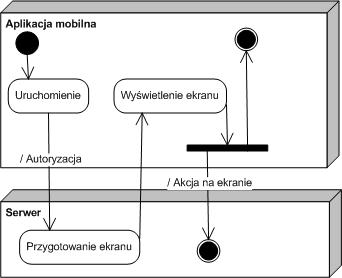
\includegraphics{img/pool_schema_uml.png} }}
\end{center}
\begin{itemize}
  \item Tworzymy nowy 'ekran' na serwerze. Oznacza to okre�lenie wygl�du i
  zachowania aplikacji w formacie XML. Okre�lamy dost�pne dla
  danego ekranu akcje. 
  \item Aplikacja mobilna ��czy si� z serwerem i pobiera przygotowany dla niej
  ekran. U�ytkownik wykonuje jedn� z dost�pnych na nim akcji, a informacja o
  tym jest przesy�ana do serwera. Dodatkowo aplikacja mo�e wykona� dowolne
  zdefiniowane akcje. W ten spos�b pojawia si� mo�liwo�� kontrolowania ekranu
  po stronie klienta w dowolny spos�b.
  \item Aplikacja mobilna pobiera kolejny ekran przygotowany przez serwer i
  dalej post�puje wed�ug powy�szego schematu.
\end{itemize}


\subsection{Mo�liwo�ci}
Aplikacja oparta o tak zaprojektowany model posiada�aby cechy typowe dla modelu
dwuwarstwowego - w tym szybki czas reakcji, niezale�no�� wygl�du aplikacji od
stosowanego klienta oraz mo�liwo�� przeprowadzenia pewnych dodatkowych operacji
(jak walidacja) po stronie klienta. W idealnym przypadku m�g�by by�
dynamicznie przesy�any kod wykonywany po stronie klienta (odpowiednik JavaScript
w przypadku przegl�darki internetowej). Pozbawiona by�aby te� typowych wad obu rozwi�za� -
brak konieczno�ci aktualizowania aplikacji przy drobnych poprawkach (poza
b��dami w zainstalowanym oprogramowaniu). Nie by�aby r�wnie� ograniczona do
mechanizm�w oferowanych przez statyczne strony WWW - mo�na by by�o
wy�wietla� dowolne ekrany, a na nich wykonywa� dowolne akcje.
Dodatkowo, poniewa� stan aplikacji przechowywany by�by na serwerze, mo�na w
dowolnym momencie zmieni� urz�dzenie mobilne, wy��czy� aplikacj�, a potem
powr�ci� do zapami�tanego wcze�niej miejsca.
 
\subsection{Dlaczego to jest nowatorskie - jak by to napisa�?}

Tworzymy aplikacj� kt�ra ma sens tylko dla urz�dze� mobilnych, zacz�tek do
tworzenia mobilnych rozwi�za�.

Post�pujemy w spos�b kt�ry nie by� nigdzie stosowany



\subsection{Mo�liwe zastosowania}
Opisywana idea u�atwia tworzenie okre�lonego typu aplikacji i tak jak ka�dy
szablon nie pokrywa wszystkich istniej�cych rozwi�za�. Nasz szablon u�atwi
pisanie aplikacji, kt�re nie wymagaj� przesy�ania du�ych ilo�ci danych i od
kt�rej oczekujemy interaktywno�ci wi�kszej ni� w przypadku strony internetowej
pozbawione JavaScript. 

\subsubsection{Ankietowanie}
Jednym z zastosowa� kt�re mo�emy sobie wyobrazi� jest zdalne ankietowanie
u�ytkownik�w. Stworzenie aplikacji kt�ra na ekranie wy�wietla list� dost�pnych
odpowiedzi i pozwala na wybranie jednej z nich, jest przy u�yciu
przedstawianego szablonu prostym zadaniem.
\subsubsection{Zdalne podejmowanie decyzji}
Podobnie jak powy�ej, u�ytkownicy mog� wybra� jedn� z mo�liwych decyzji, w
takim przypadku potrzebne b�dzie rozbudowanie szablonu o zaawansowane
mechanizmy bezpiecze�stwa, jednak idea pozostaje podobna.
\subsubsection{Zdalne wy�wietlanie tre�ci}
Urz�dzenie mobilne mo�e by� te� jedynie miejscem kt�re wy�wietla dostarczane do
niego informacje. Interakacja z u�ytkownikiem mo�e by� w tym momencie
wy��czona, a urz�dzenie mobilne mo�e 




\subsection{Architektura}
Tak jak zosta�o to ju� wspomniane szablon sk�ada si� z dw�ch
g��wnych cz�ci - serwerowej oraz mobilnej. Przed przej�ciem do szczeg��w
implementacyjnych zaprezentujemy koncepcj� ca�ego systemu.

\setlength\fboxsep{5pt}  
\setlength\fboxrule{0.0pt}
\begin{center}
\fbox{\scalebox{0.7}{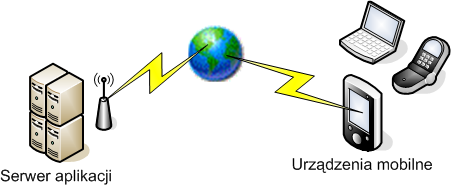
\includegraphics{img/diag1.png} }}
\end{center}
Jak wida�, urz�dzenia mobilne b�d� si� ��czy�y przez Internet do uruchomionego
serwera aplikacyjnego. Ka�de z nich wysy�a ��danie pobrania ekranu, kt�ry jest
dynamicznie przygotowywany w zale�no�ci od stanu aplikacji dla danego
u�ytkownika. Warto tu zwr�ci� uwag�, �e szablon jest pomy�lany w�a�ciwie
wy��cznie dla urz�dze� mobilnych - stosowane rozwi�zania, s� albo niedost�pne,
albo ma�o przydatne w przypadku komputer�w stacjonarnych, o czym napiszemy
w dalszej cz�ci pracy. 
\newline
Podczas projektowania szablonu pojawi�y si� w�tpliwo�ci co do sposobu
komunikacji pomi�dzy elementami systemu. Pocz�tkowa i bardzo przekonuj�ca
koncepcja zak�ada�a wykorzystanie JMS - Java Messaging System, specyfikacji
umo�liwaj�cej przesy�anie wiadomo�ci w Javie. Przemawia� za tym szereg
argument�w:
\begin{itemize}
  \item Niezawodno�� - gwarancja dostarczenia wiadomo�ci w warunkach ��czno�ci
  bezprzewodowej, kt�ra jest szczeg�lnie nara�ona na przerwy w transmisji.
  \item Niezale�no�� system�w - u�ycie wiadomo�ci znacznie u�atwi�oby
  ewentualne zmiany po stronie serwera aplikacyjnego, ze wzgl�du na dodatkowy
  element po�rednicz�cy jakim jest serwer wiadomo�ci.
  \item �atwo�� implementacji - przesy�ane wiadomo�ci mog� zawiera�
  zserializowane obiekty, co zdejmuje z programisty obowi�zek samodzielnej
  serializacji i deserializacji danych.
\end{itemize}
Jak si� jednak okaza�o,istotne ograniczenia techniczne po stronie urz�dze�
mobilnych uniemo�liwi�y skorzystanie z JMS. Jest to technologia wymagaj�ca
znacznych zasob�w, niedost�pnych w specyfikacji Java Micro Edition - platformy
na kt�rej stworzyli�my nasz szablon. Nie daje ona mo�liwo�ci bezpo�redniego
pod��czenia do kana�u komunikacyjnego, co wymusza korzystanie z zewn�trznych
bibliotek. Jednak nawet wtedy, okazuje si�, �e takie biblioteki korzystaj� z
Web Serwis�w jako technologii po�rednicz�cej w komunikacji. Podobnie,
automatyczna serializacja i deserializacja w takiej sytuacji nie jest jeszcze
wspierana. 
\newline
Z tych powod�w zdecydowali�my si� na wykorzystanie Web serwis�w jako warstwy
komunikacyjnej i samodzielne rozwi�zanie problem�w, kt�re si� z tym wi���.



\subsubsection{Aplikacja serwerowa}

Przedstawimy teraz architektur� cz�ci serwerowej, komponenty z kt�rych si�
sk�ada i technologie, kt�re wykorzystuj�.
\newline
Aby zrozumie� projekt ca�ego systemu wprowad�my pewne poj�cia w naszym
systemie, z kt�rych wynikaj� dalsze rozwi�zania: 
\begin{itemize}
  \item \emph{Ankieta} - tre��, dla kt�rej istniej� dost�pne zdefiniowane
  odpowiedzi.
 \item \emph{Odpowied�} - jedna z mo�liwo�ci wyboru dost�pnych dla danej ankiety
  \item \emph{U�ytkownik} - konto z kt�rym zwi�zane s� uprawnienia i udzielone
  w ankietach odpowiedzi. Jeden u�ytkownik mo�e udzieli� wielu odpowiedzi w
  trakcie dzia�ania ca�ego systemu.
\end{itemize}
\setlength\fboxsep{5pt}  
\setlength\fboxrule{0.0pt}

Aplikacja serwerowa zbudowana zosta�a w oparciu o model tr�jwarstwowy, z
podw�jnym dost�pem (widokiem) do danych. 

\begin{center}
\fbox{\scalebox{0.7}{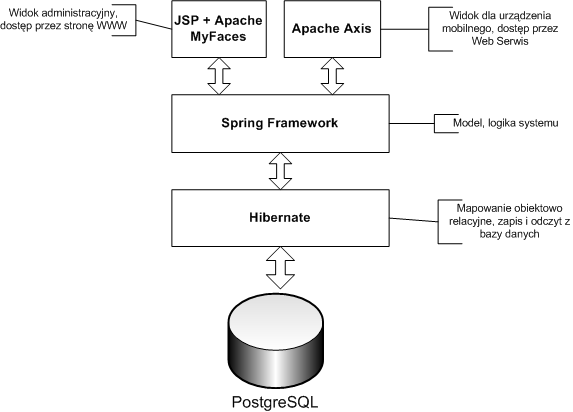
\includegraphics{img/diag2.png} }}
\end{center}
Przedstawmy teraz poszczeg�lne warstwy systemu, wraz z przyj�tymi w nich
za�o�eniami.

\paragraph{Serwer}
Aplikacja serwerowa jest uruchamiana na kontenerze Apache Tomcat 6.0.

\paragraph{Baza danych}
W oparciu o przedtawione wcze�niej za�o�enia stworzony zosta� prosty schemat
bazy danych:
\begin{center}
\fbox{\scalebox{0.7}{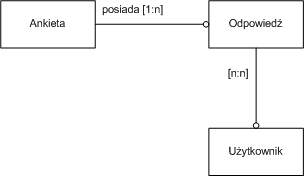
\includegraphics{img/pool_schema_o.png} }}
\end{center}
Cho� wydaje si�, �e ogranicza to dzia�anie systemu do mo�liwo�ci wyboru
odpowiedzi z dost�pnej listy, to jednak schemat bez problemu mo�na rozbudowa� o
dodatkowe pola, kt�re pozwol� na podawanie wolnych (nieograniczonych dost�pn�
list� wyboru) odpowiedzi.
\newline
Na postawie schematu koncepcyjnego stworzony zosta� schemat fizyczny bazy
danych:
\newline
\begin{center}
\fbox{\scalebox{0.7}{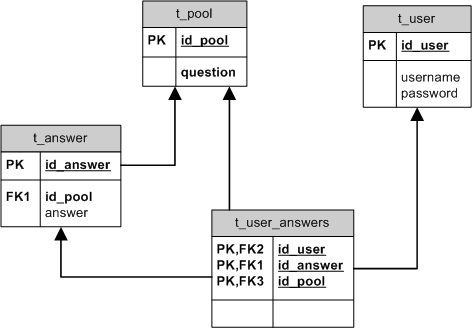
\includegraphics{img/pool_schema.png} }}
\end{center}


\paragraph{Hibernate}
Dost�p do danych realizowany jest za pomoc� mapowania relacyjno-obiektowego
Hibernate. Teoretycznie pozwala to, a na pewno znacznie u�atwia ewentualn�
zmian� dostawcy bazy danych. Dodatkowo uwalnia nas z konieczno�ci r�cznego
pisania zapyta� SQL. 

\paragraph{Spring Framework}
Spring jest zestawem narz�dzi u�atwiaj�cym tworzenie aplikacji. Pozwala on,
mi�dzy innymi, na deklaratywne zarz�dzanie transakcjami, zarz�dzanie czasem
cyklem �ycia obiekt�w oraz zwalnia programist� z konieczno�ci pisania
 cz�sto powtarzanego kodu przez dostarczenie odpowiednich szablon�w. Dodatkowo
 wymusza on pewien model programowania i sprawia, �e pisane aplikacje s�
 bardziej przejrzyste i �atwiejsze w utrzymaniu. Jak ju� zosta�o to wspomniane
 aplikacja serwerowa jest aplikacj� typu Web, z kt�r� to framework Spring
 doskonale si� integruje.
 
\paragraph{Apache Myfaces} 
Myfaces jest implementacj� specyfikacji Java Server Faces, kt�ra pozwala na
wygodne tworzenie widoku aplikacji. W naszym przypadku interfejsem b�dzie
dynamicznie generowana strona WWW, cho� specyfikacja JSF nie wprowadza takiego
ograniczenia. Warstwa ta b�dzie s�u�y�a do administrowania systemem,
przegl�dania podj�tych decyzji i zarz�dzania ankietami i u�ytkownikami.

\paragraph{Apache Axis2}
Axis2 to kontener webserwis�w,kt�ry odpowiada za odbieranie zdalnych wywo�a�
procedur i przekazywanie ich do odpowiednich obiekt�w kt�re je wykonuj�.
Zwalnia te� programist� z konieczno�ci samodzielnego przetwarzania XML w
��daniach, umo�liwia te� automatyczn� serializacj� i deserializacj� obiekt�w
Javowych. 

\paragraph{Transformata XSLT}
Elementem wspomagaj�cym w systemie jest transformata XSLT wykonywana na
odpowiedziach przesy�anych do urz�dzenia mobilnego. Jej celem jest utworzenie
widoku dla urz�dzenia mobilnego w spos�b niezale�ny od generowanej odpowiedzi.
W wyniku wywo�ania procedury generuj�cej ekran, tworzony jest XML, zawieraj�cy
podstawowe informacje, a nast�pnie przetwarzany jest on w opisany spos�b,
dzi�ki czemu odpowied� mo�na dowolnie modyfikowa� bez zmiany kodu aplikacji.

\subsubsection{Aplikacja mobilna}

\subsection{Istniej�ce problemy}

\subsubsection{Bezpiecze�stwo}

\subsubsection{Gwarancja dostarczenia}

\subsubsection{Transakcyjno��}
\chapter{Mobilny system informacyjny}


\section{Interfejs mobilny}


\section{Interfejs administracyjny}

\begin{thebibliography}{99}
\bibitem{Entj2me} Michael Juntao Yuan: \emph{Enterprise J2ME Developing Mobile
Applcations}, Prentice Hall Pennsylvania 2004
\bibitem{Entpatterns} Gregor Hophe,Bobby Woolf: \emph{Enterprise Integration
Patterns}, The Addison-Wesley Signaure Series 2003
\bibitem{j2me} Kim: Topley \emph{J2ME. Almanach}, Helion O'REILLY 2003
\bibitem{techfaq360}: \emph{Spring Tutorial},
http://www.techfaq360.com/tutorial/spring/
\bibitem{WebServicesIBM}: \emph{Which WSDL},
http://www.ibm.com/developerworks/webservices/\\library/ws-whichwsdl/
\bibitem{computerwoche} Karin Quack: \emph{Die gro�en Herausforderungen},
Computerwoche 26.03.2008
\bibitem{omapach} \emph{O mapach},
http://gps.put.mielec.pl/mapy.htm
\bibitem{operadevelop} \emph{Opera mobile - developer angle},
http://dev.opera.com/articles/view/\\opera-mobile-9-5-the-developer-angle/
\bibitem{bbdev} \emph{Java development for Blackberry},
http://na.blackberry.com/eng/developers/\\javaappdev/
\bibitem{kuix} \emph{Kuix Framework Home Page},
http://www.kalmeo.org/projects/kuix
\bibitem{j2megui} \emph{List of available GUI frameworks for Java Micro
Edition},
http://newsofthefuture.net/\\index.php?/archives/33-Evaluation-GUI-libraries-for-J2ME.html
\bibitem{bbsecurity} \emph{Blackberry security}
http://na.blackberry.com/eng/ataglance/security/\\features.jsp
\bibitem{jmsnj2me} Martin Erzberger: \emph{Using JMS and J2ME for Building
Interactive Mobile Applications}, Softwired AG, Z�rich 
\end{thebibliography}
\end{document}
 